\chapter{Cryptocurrency Exchanges}
\label{ch:exchanges}

In dit hoofdstuk beschrijven we verschillende cryptocurrency exchanges - online marktplaatsen - met de belangrijkste bijbehorende eigenschappen in meer detail. Daarnaast geven we een voorselectie van verschillende bekende exchanges. Er wordt behandeld waar je op moet letten als je een exchange gaat gebruiken, cryptocurrencies gaat kopen, verkopen en traden, en er wordt uitgelegd welke stappen iemand kan nemen om zelf een account aan te maken. We beginnen bij de basis.

\medskip

\section{Wat zijn cryptocurrency exchanges}
Een cryptocurrency exchange is een online marktplaats (handelsplatform) waar je cryptocurrencies kunt kopen, verkopen en traden tegen andere cryptocurrencies. Op een aantal exchanges kan met (digitale) fiat currencies, zoals de US Dollar of de euro, cryptocurrencies gekocht worden. Wie professioneel wil starten en toegang wil tot handige trading tools bij het traden, zal in de meeste gevallen een bekende - en gereguleerde - exchange moeten gebruiken waarbij iemands ID moet worden gecontroleerd. Dit proces noemt men \emph{Know Your Customer} (KYC). Hierbij wordt jouw identiteit geverifieerd en open je een eigen account op het desbetreffende platform. Er zijn twee verschillende type cryptocurrency exchanges die je kunt gebruiken om te traden en cryptocurrencies te kopen.\medskip

\begin{enumerate}[label=(\alph*)]
  \setlength\itemsep{0em}
    \item Broker Exchanges (\cref{subsec:broker_exchange})
        \begin{itemize}
            \item Veelal gecentraliseerd, hoofdzakelijk om crypto te kopen met fiat currency (\cref{subsubsec:CEX}).
        \end{itemize}
    \item Trading Exchanges (\cref{subsec:trading_exchange})
        \begin{itemize}
            \item Zowel gecentraliseerd als gedecentraliseerd, hoofdzakelijk om crypto te traden. Tegenwoordig kan je bij een aantal ook direct kopen met fiat currency (\cref{subsubsec:DEX}).       
            \end{itemize}
\end{enumerate}

Het is belangrijk de verschillen tussen de exchanges te begrijpen. Dit vormt de eerste essenti{\"e}le stap om de geschikte cryptocurrency exchange voor jezelf te kiezen. Voordat de verschillen tussen exchanges worden behandeld, zullen de belangrijke aspecten van het koop- en verkoopproces in het algemeen worden besproken.


\subsection*{Kopen en verkopen van cryptocurrency}
Cryptocurrency exchanges hebben net als alle andere exchanges en markten te maken met [il]liquiditeit. De liquiditeit beschrijft de mate waarin een bezit of middel snel op de markt kan worden gekocht of verkocht zonder de prijs van het bezit of middel te be{\"i}nvloeden. De cryptocurrency markt zelf is zeer volatiel en telt een paar relatief liquide cryptocurencies. Een liquide cryptocurrency is gemakkelijk snel te verkopen vanwege de talrijke beschikbare en bereidwillige kopers. Een illiquide cryptocurrency is lastig te verkopen en heeft vaak een laag handelsvolume en een kleine marktkapitalisatie.\medskip 

 Liquide middelen zijn relatief eenvoudig te kopen en te verkopen en de meerderheid van de mensen en bedrijven accepteert liquide middelen als betaalmiddel.
 
    \bigskip
    \begin{cryptobox}{LIQUID CASH}
        \textit{Het beste voorbeeld van een liquide middel is contant geld. Iedereen accepteert contant geld en het kan bijna overal ter wereld gebruikt worden. Bij een internationale reis moet je wellicht wel je contant geld omwisselen in de nationale valuta al naargelang jouw bestemming. Doordat contant geldmarkten zo liquide zijn, kennen ze weinig tot geen volatiliteit in de wisselkoersen van dag tot dag.}
    \end{cryptobox}
    \medskip
    
Er zijn duizenden cryptocurrency projecten, maar tegelijkertijd zijn er talloze exchanges waar al deze activa worden verkocht, wat een deel van het probleem vormt. In principe concurreren de exchanges met elkaar om liquiditeit en handelsvolume in een nog relatief kleine markt dat een relatief lage marktkapitalisatie heeft.

\section{Verschillende soorten exchanges}
\label{sec:exchangetypes}

Er zijn tal van exchanges beschikbaar die in jouw geografische locatie opereren. Als je ge{\"i}nteresseerd bent in de aankoop van een bepaalde cryptocurrency, kun je gebruikmaken van plaforms zoals CoinMarketCap en CoinGecko zoals weergegeven in \cref{tab:exchangeoverview}.
Daar navigeer je dan naar de specifieke cryptocurrency of exchange en krijg je toegang tot een wereld van informatie die je zelf kunt gaan filteren. Dit overzicht is waardevol voor wie op zoek is naar populaire exchanges, exchanges met een hoog volume, exhanges die veel cryptocurrencies aanbieden, of die al jaren bestaan. Kortom, dergelijke geaggregeerde sites zijn een ideale plek om de cryptocurrency markt en de projecten op de markt te verkennen en te onderzoeken.


\begin{table}

\centering

\caption{Websites met informatie over exchanges}
\begin{tabular}{ll} 
\toprule

\textbf{Platform} & \textbf{URL}\\
\midrule

CoinMarketCap   & \href{https://coinmarketcap.com}{coinmarketcap.com}      \\
CoinGecko       & \href{https://www.coingecko.com/en}{coingecko.com}    \\
CoinCheckup & \href{https://coincheckup.com}{coincheckup.com}    \\
CryptoCompare   & \href{https://www.cryptocompare.com}{cryptocompare.com}  \\
CoinPaprika      & \href{https://coinpaprika.com}{coinpaprika.com}         \\


\bottomrule
\end{tabular}
\label{tab:exchangeoverview}
\end{table}

\medskip

\subsection{Broker exchanges: van fiat- naar cryptocurrency}
\label{subsec:broker_exchange}

Een broker exchange zet fiat currencies, zoals de euro, effectief om naar cryptocurrencies. Of andersom, je crypto terug converteren naar fiat currency. Een broker exchange is vereist voor beginners en vormt het startpunt als je nog geen cryptocurrencies heb gekocht welke je kunt verhandelen. 

\bigskip
\begin{cryptobox}{WAT IS FIAT?}
        Fiat currency is een valuta die bestaat bij het dictaat of door fiat van een regering en/of bank. Fiat is een Latijns woord voor een valuta die opgelegd in omloop is. 
        Modern papiergeld en munten zijn, samen met hun digitale tegenhanger, enigszins duurzaam in waarde; fiat valuta  kan echter niet langer aanspraak maken op enige intrinsieke waarde. De waarde ervan wordt ervaren op basis van geloof en vertrouwen, en dat vertrouwen komt voort uit de steun van de respectieve overheden en een nationaal of internationaal vertrouwen in de stabiliteit van de munt. Geen enkele regering of bank heeft ooit haar monetaire beleid kunnen disciplineren. Door de gehele geschiedenis heeft geen enkele fiat valuta het overleefd, en zijn allen naar een waarde van nul gegaan. %\parencite{thebigreset}
\end{cryptobox}
\bigskip

Nederlandse exchanges slaan wij momenteel over vanwege de hoge transactiekosten en het hanteren van relatief hogere cryptocurrency prijzen vergeleken met internationale spelers.


\subsubsection*{Coinbase (CEX)}
Coinbase is zonder twijfel {\'e}{\'e}n van de bekendste exchanges ter wereld. Coinbase behoort tot de grootste broker exchanges, zeer gebruiksvriendelijk voor beginners, maar rekent relatief hoge transactiekosten. Bij Coinbase kun je de bekendste cryptocurrencies zoals Bitcoin en Ethereum kopen en verkopen door je simpelweg te registreren, je bankrekening te koppelen en een storting te doen. Je kunt stortingen doen in ontzettend veel fiat currencies. Zodra je rekening is gecrediteerd, ontvang je een e-mailbericht dat je de vers gestorte euro's kunt inwisselen voor een cryptocurrency naar keuze. De website biedt meerdere online wallets aan waarin cryptocurrencies kunnen worden opgeslagen en bewaard. Van hieruit kun je betalingen versturen en ontvangen.\medskip

\begin{topbox}{Top}
Meld je aan bij \href{https://www.coinbase.com/join/51954a2b26a1bcc484000015}{Coinbase} via {\fontseries{extrabold}\selectfont cryptomanuals} en ontvang bij een storting van \euro 100 direct \euro 8 aan gratis Bitcoin!
\tcblower
Meer weten? Kijk op \href{https://support.coinbase.com/}{Coinbase Support}.
\end{topbox}

\begin{borderbox}
    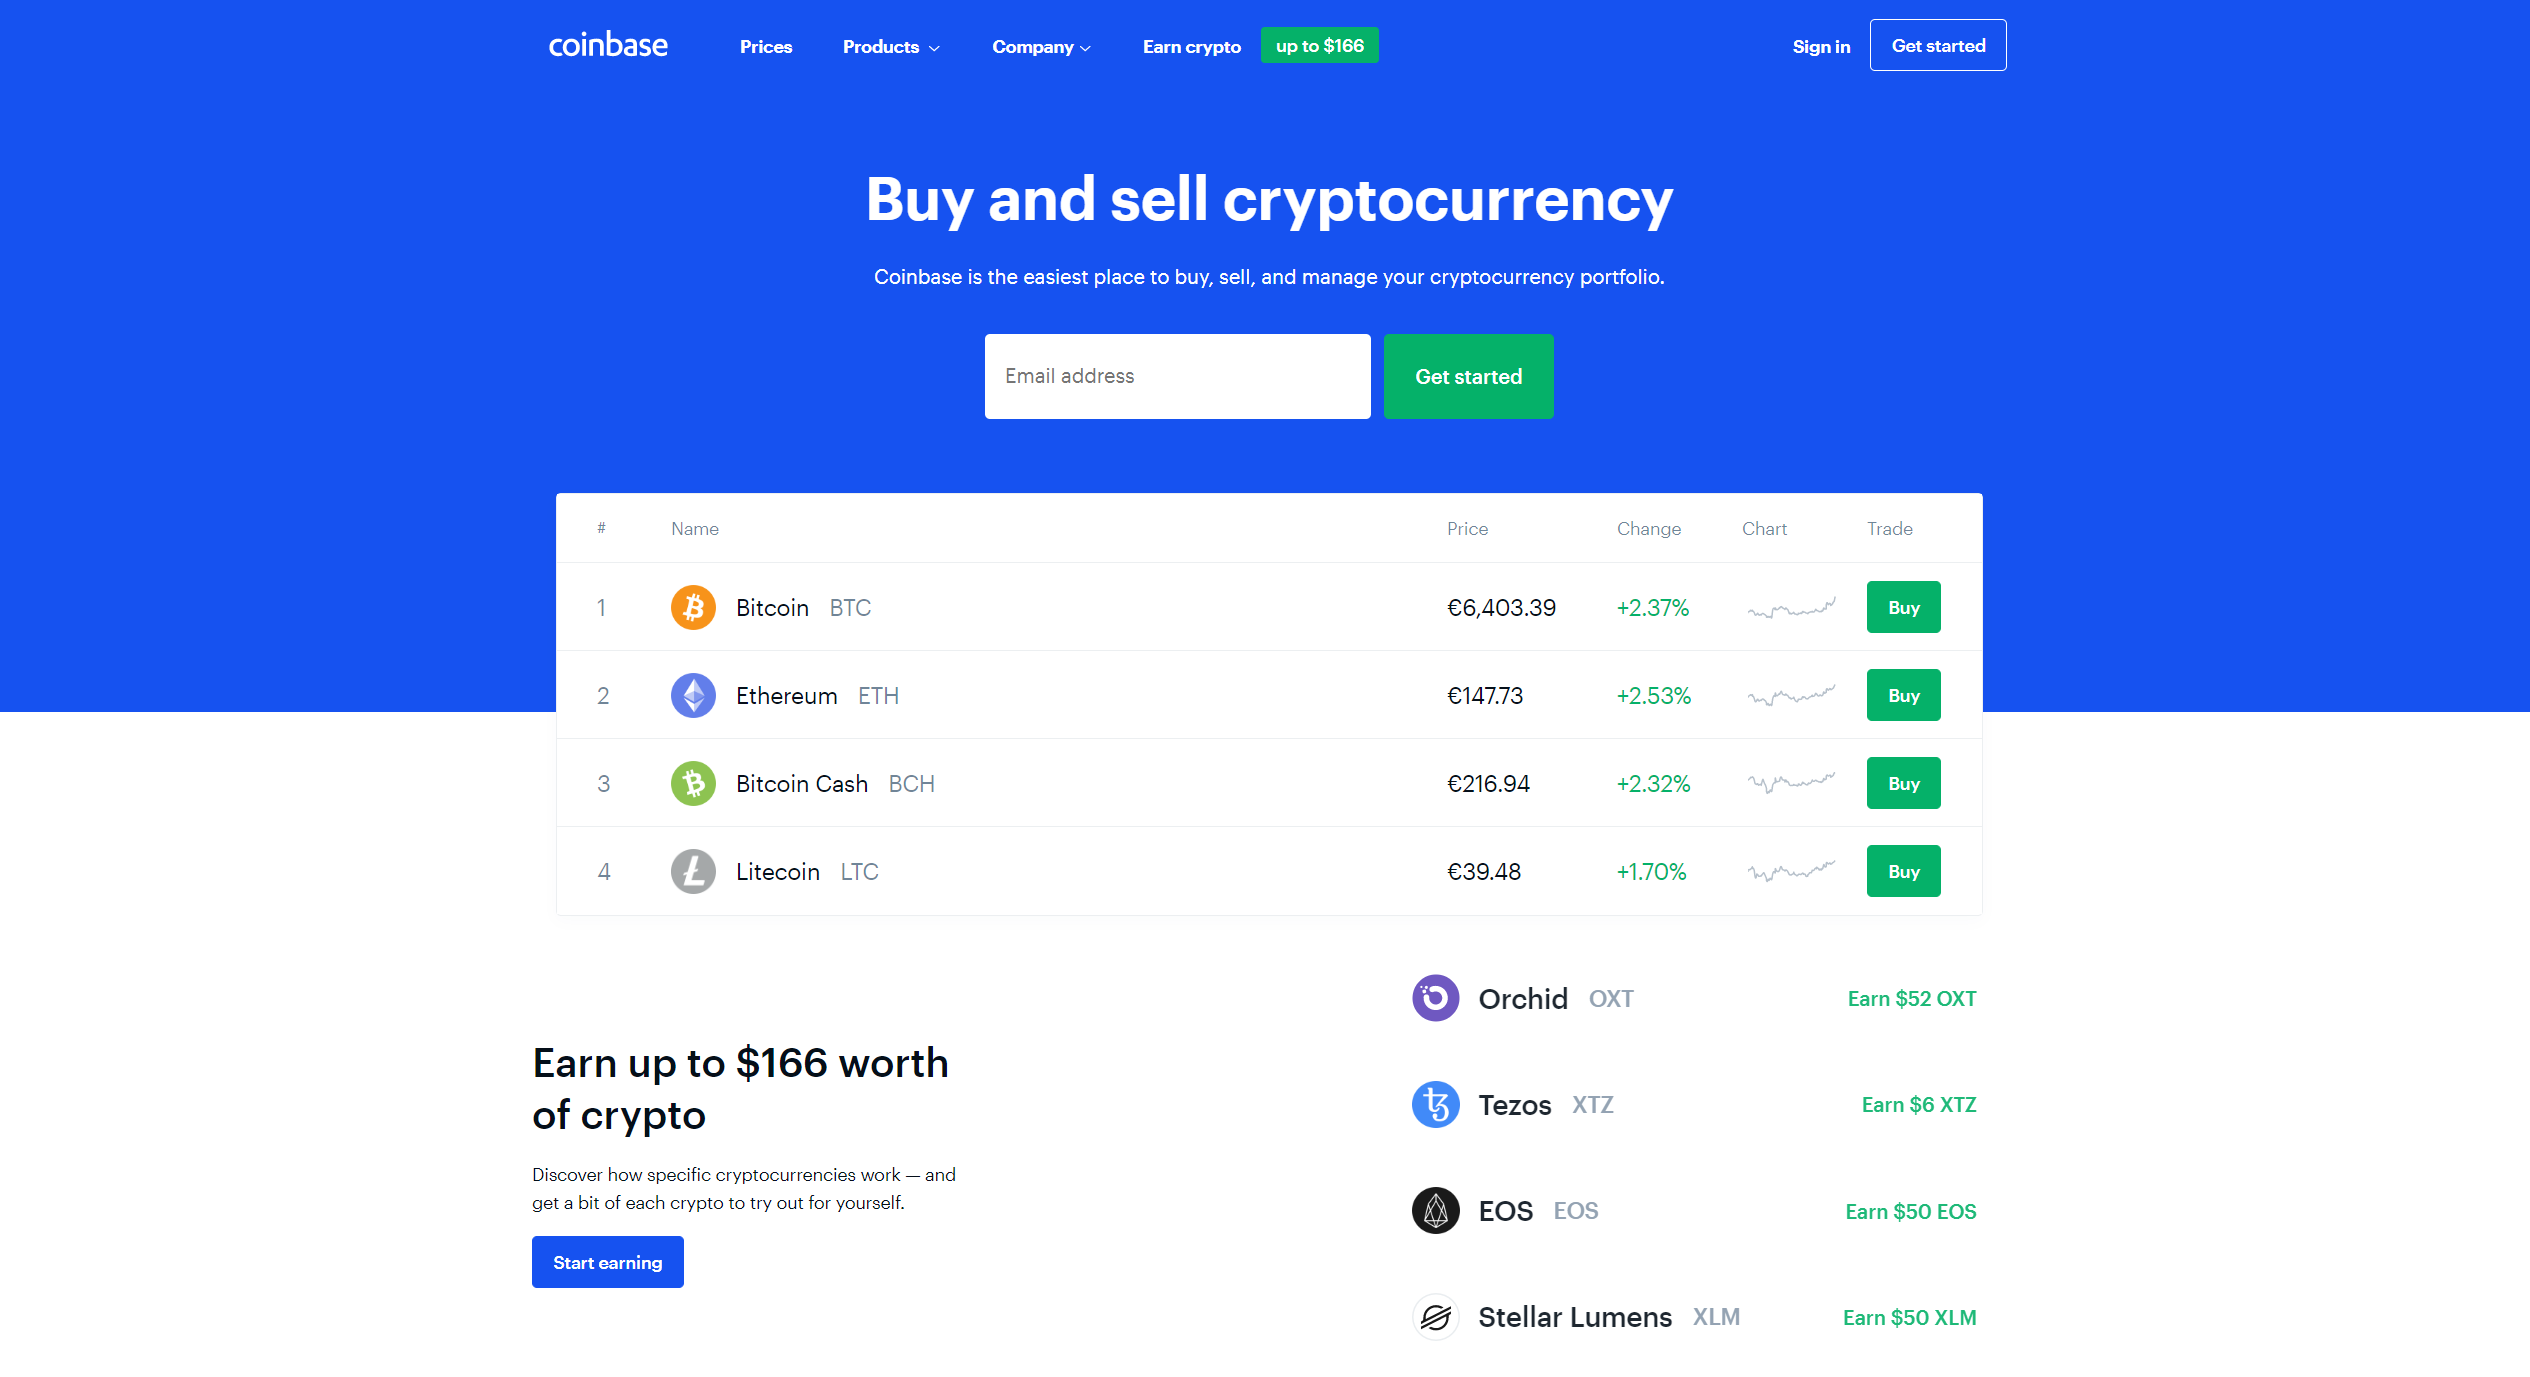
\includegraphics[width=\textwidth]{img/ch-exchanges/coinbase.png}
\end{borderbox}

\subsubsection*{Kraken (CEX)}
\href{https://www.kraken.com/}{Kraken} werd opgericht in 2011 en staat bekend als {\'e}{\'e}n van de grootste en oudste Bitcoin-exchanges ter wereld. Kraken wordt consequent genoemd als {\'e}{\'e}n van de beste plaatsen om crypto online te kopen en te verkopen. Het heeft onlangs de website en UI/UX-interfaces ge{\"u}pdate en probeert een groter publiek aan te spreken. 

\subsubsection*{Bitvavo (CEX)}
Voor een Nederlandse speler op de markt kun je bij \href{https://bitvavo.com/nl}{Bitvavo} terecht. Het platform leent zicht voor beginnende en ervaren traders. Ze bieden 50 digitale valuta aan en vragen maximaal 0.25\% handelskosten. Het heeft een eenvoudige interface voor beginnende traders en een geavanceerde interface voor ervaren traders.
 
\subsubsection*{Liquid (CEX)}
 Liquid is een wereldwijd opererend handelsplatform dat een brug slaat tussen de wereld van fiat en cryptocurrencies. Het is een platform dat een hoge mate van liquiditeit biedt door middel van hun \say{World Book}, dat de liquiditeitspools van exchanges over de hele wereld met elkaar verbindt. Ze bieden ook een breed scala aan deposito's en opnames in fiat currency en hanteren zeer lage transactiekosten. Bovendien zijn ze volledig gereguleerd en bieden ze een zeer intu{\"i}tieve gebruikersinterface en gebruikerservaring. Dankzij hun eigen interne token QASH geniet je daarnaast van 50\% handelskortingen.\medskip

\begin{topbox}{Top}
Bij \href{https://www.liquid.com?affiliate=nUfQhVL4164547}{Liquid} kan je jouw cryptocurrency op een veilige manier uitlenen aan anderen. Daarnaast biedt Liquid fiat currency conversie aan en is volledig gereguleerd. De trading fees zijn erg laag en er is snelle opname van crypto of fiat currency.
\end{topbox}

\begin{table}[b]

\centering

\caption{Aanbevolen broker and trading exchanges}
\begin{tabular}{llll} 
\toprule

\textbf{Exchange} & \textbf{Type } & \textbf{UX/UI} & \textbf{URL}\\
\midrule

Coinbase & Broker & Beginner & \href{https://www.coinbase.com/join/51954a2b26a1bcc484000015}{coinbase.com} \\
KuCoin   &  Trading & Beginner & \href{https://www.kucoin.com/#/?r=aNuPeb}{kucoin.com} \\
Binance  &  Broker/Trading & Intermediate & \href{https://www.binance.com/?ref=35602166}{binance.com} \\
Liquid   &  Broker/Trading & Beginner & \href{https://www.liquid.com?affiliate=nUfQhVL4164547}{liquid.com} \\
Kraken   &  Broker/Trading & Intermediate & \href{https://www.kraken.com/}{kraken.com} \\


\bottomrule
\end{tabular}
\label{tab:exchange selection}
\end{table}

\subsection{Trading exchanges: van crypto naar crypto}
\label{subsec:trading_exchange}

Dit type exchange vormt de brug naar de wereld van altcoins (een verzamelbegrip voor alle coins buiten Bitcoin). Hier kun je namelijk gemakkelijk en snel cryptocurrencies verhandelen voor andere cryptocurrencies. Als je bijvoorbeeld in het bezit bent van Ethereum en je wilt graag andere Altcoins kopen, dan kun je een deel van de Ethereum voor iets anders verkopen met behulp van een account op een trading exchange. Een trading exchange kan een gecentraliseerde of gedecentraliseerde exchange zijn. We noemen er een paar in de onderstaande paragrafen en geven daarbij aan of ze ge(de)centraliseerd zijn. Vergeet niet dat dit slechts enkele voorbeelden zijn - raadpleeg voor een volledig overzicht een van de bronnen in \cref{tab:exchangeoverview}.

\bigskip

\begin{tipbox}{Tip}
          Tegenwoordig kun je bij steeds meer voormalige trading-only exchanges ook direct crypto aanschaffen met bijvoorbeeld iDEAL (Binance). Andersom geldt ook: bij een broker exchange kun je tegenwoordig ook meer dan alleen Bitcoin en Ethereum kopen, maar het aanbod is vaak veel beperkter. Voor het echte grote aanbod moet je dus naar een trading exchange.
\end{tipbox}

\subsubsection*{Binance (CEX)} 
\href{https://www.binance.com/?ref=35602166}{Binance} is {\'e}{\'e}n van de grootste en meest populaire exchanges. Het heeft een enorm handelsvolume en een grote hoeveelheid aan cryptocurrency handelsparen. Het  biedt ook een partner programma aan dat commissies aanbiedt over de transacties die door de verworven inschrijvingen worden uitgevoerd. 
Bovendien biedt het veel kwaliteitsvolle tokens, heeft het een zeer actieve en betrokken community en biedt het veel tradingtools aan om mee te traden. Het besteedt een aanzienlijk deel van zijn budget aan marketing en promotie. Het is dan ook niet verwonderlijk dat het {\'e}{\'e}n van de grootste en snelst groeiende exchanges is met een groot potentieel voor de toekomst. Daarnaast ontwikkelt Binance momenteel ook een DEX.


\subsubsection*{KuCoin (CEX)}
\href{https://www.kucoin.com/#/?r=aNuPeb}{KuCoin} is een relatief nieuwe speler die je qua gemak kunt vergelijken met Binance. Kucoin heeft trading stimulansen, die 90\% van de trading fees herverdeelt  met zijn gebruikers, promotors en investeerders. Het is een competitieve scale-up met een hoofdkantoor in Hong Kong. KuCoin heeft een strak design, UI/UX interfaces en een interessant business model. \medskip

    \begin{topbox}{Top}
    KuCoin keert dagelijks dividendbonussen uit aan KuCoin Shares (KCS) houders. Dit dividend bestaat uit een groot deel van alle transactie fees van die dag, naar rato verdeeld over iedereen met KCS op het platform.
    \tcblower
    Weten hoeveel je ontvangt bij wat voor investering? Ga naar \href{https://www.stakingrewards.com/asset/kucoin-shares}{stakingrewards}
    \end{topbox}



\subsubsection*{Changelly of ShapeShift (CEX)}
Cryptocurrency swap platforms zoals \href{https://changelly.com/?ref_id=7tas7fubzklk9f74}{Changelly} en \href{https://shapeshift.com}{ShapeShift} bieden een uitermate handige manier die sterk gericht is op gebruikerservaring, ontwerp, en veiligheid. Je kiest de te verkopen en aan te kopen crypto uit en je kunt gelijk swappen. Recentelijk ook geen fees meer op het ShapeShift platform, ideaal dus! 

\paragraph{Changelly} is een instant cryptocurrency exchange die het mogelijk maakt om snel crypto met crypto te ruilen en bovendien aan te kopen via creditcard. Changelly biedt lage crypto-naar-crypto tarieven en ondersteunt meer dan 150 cryptocurrencies.

\paragraph{ShapeShift} is het enige cryptocurrency trading platform dat \say{zero-commission} crypto trading aanbiedt {\'e}n waar de keys volledig in eigen beheer zijn. ShapeShift stelt gebruikers in staat om crypto te kopen met fiat, te handelen en hun crypto te beveiligen via een eenvoudige en mooie web-interface. Gebruikers blijven altijd de controle houden over hun sleutels.\medskip

\begin{borderbox}
     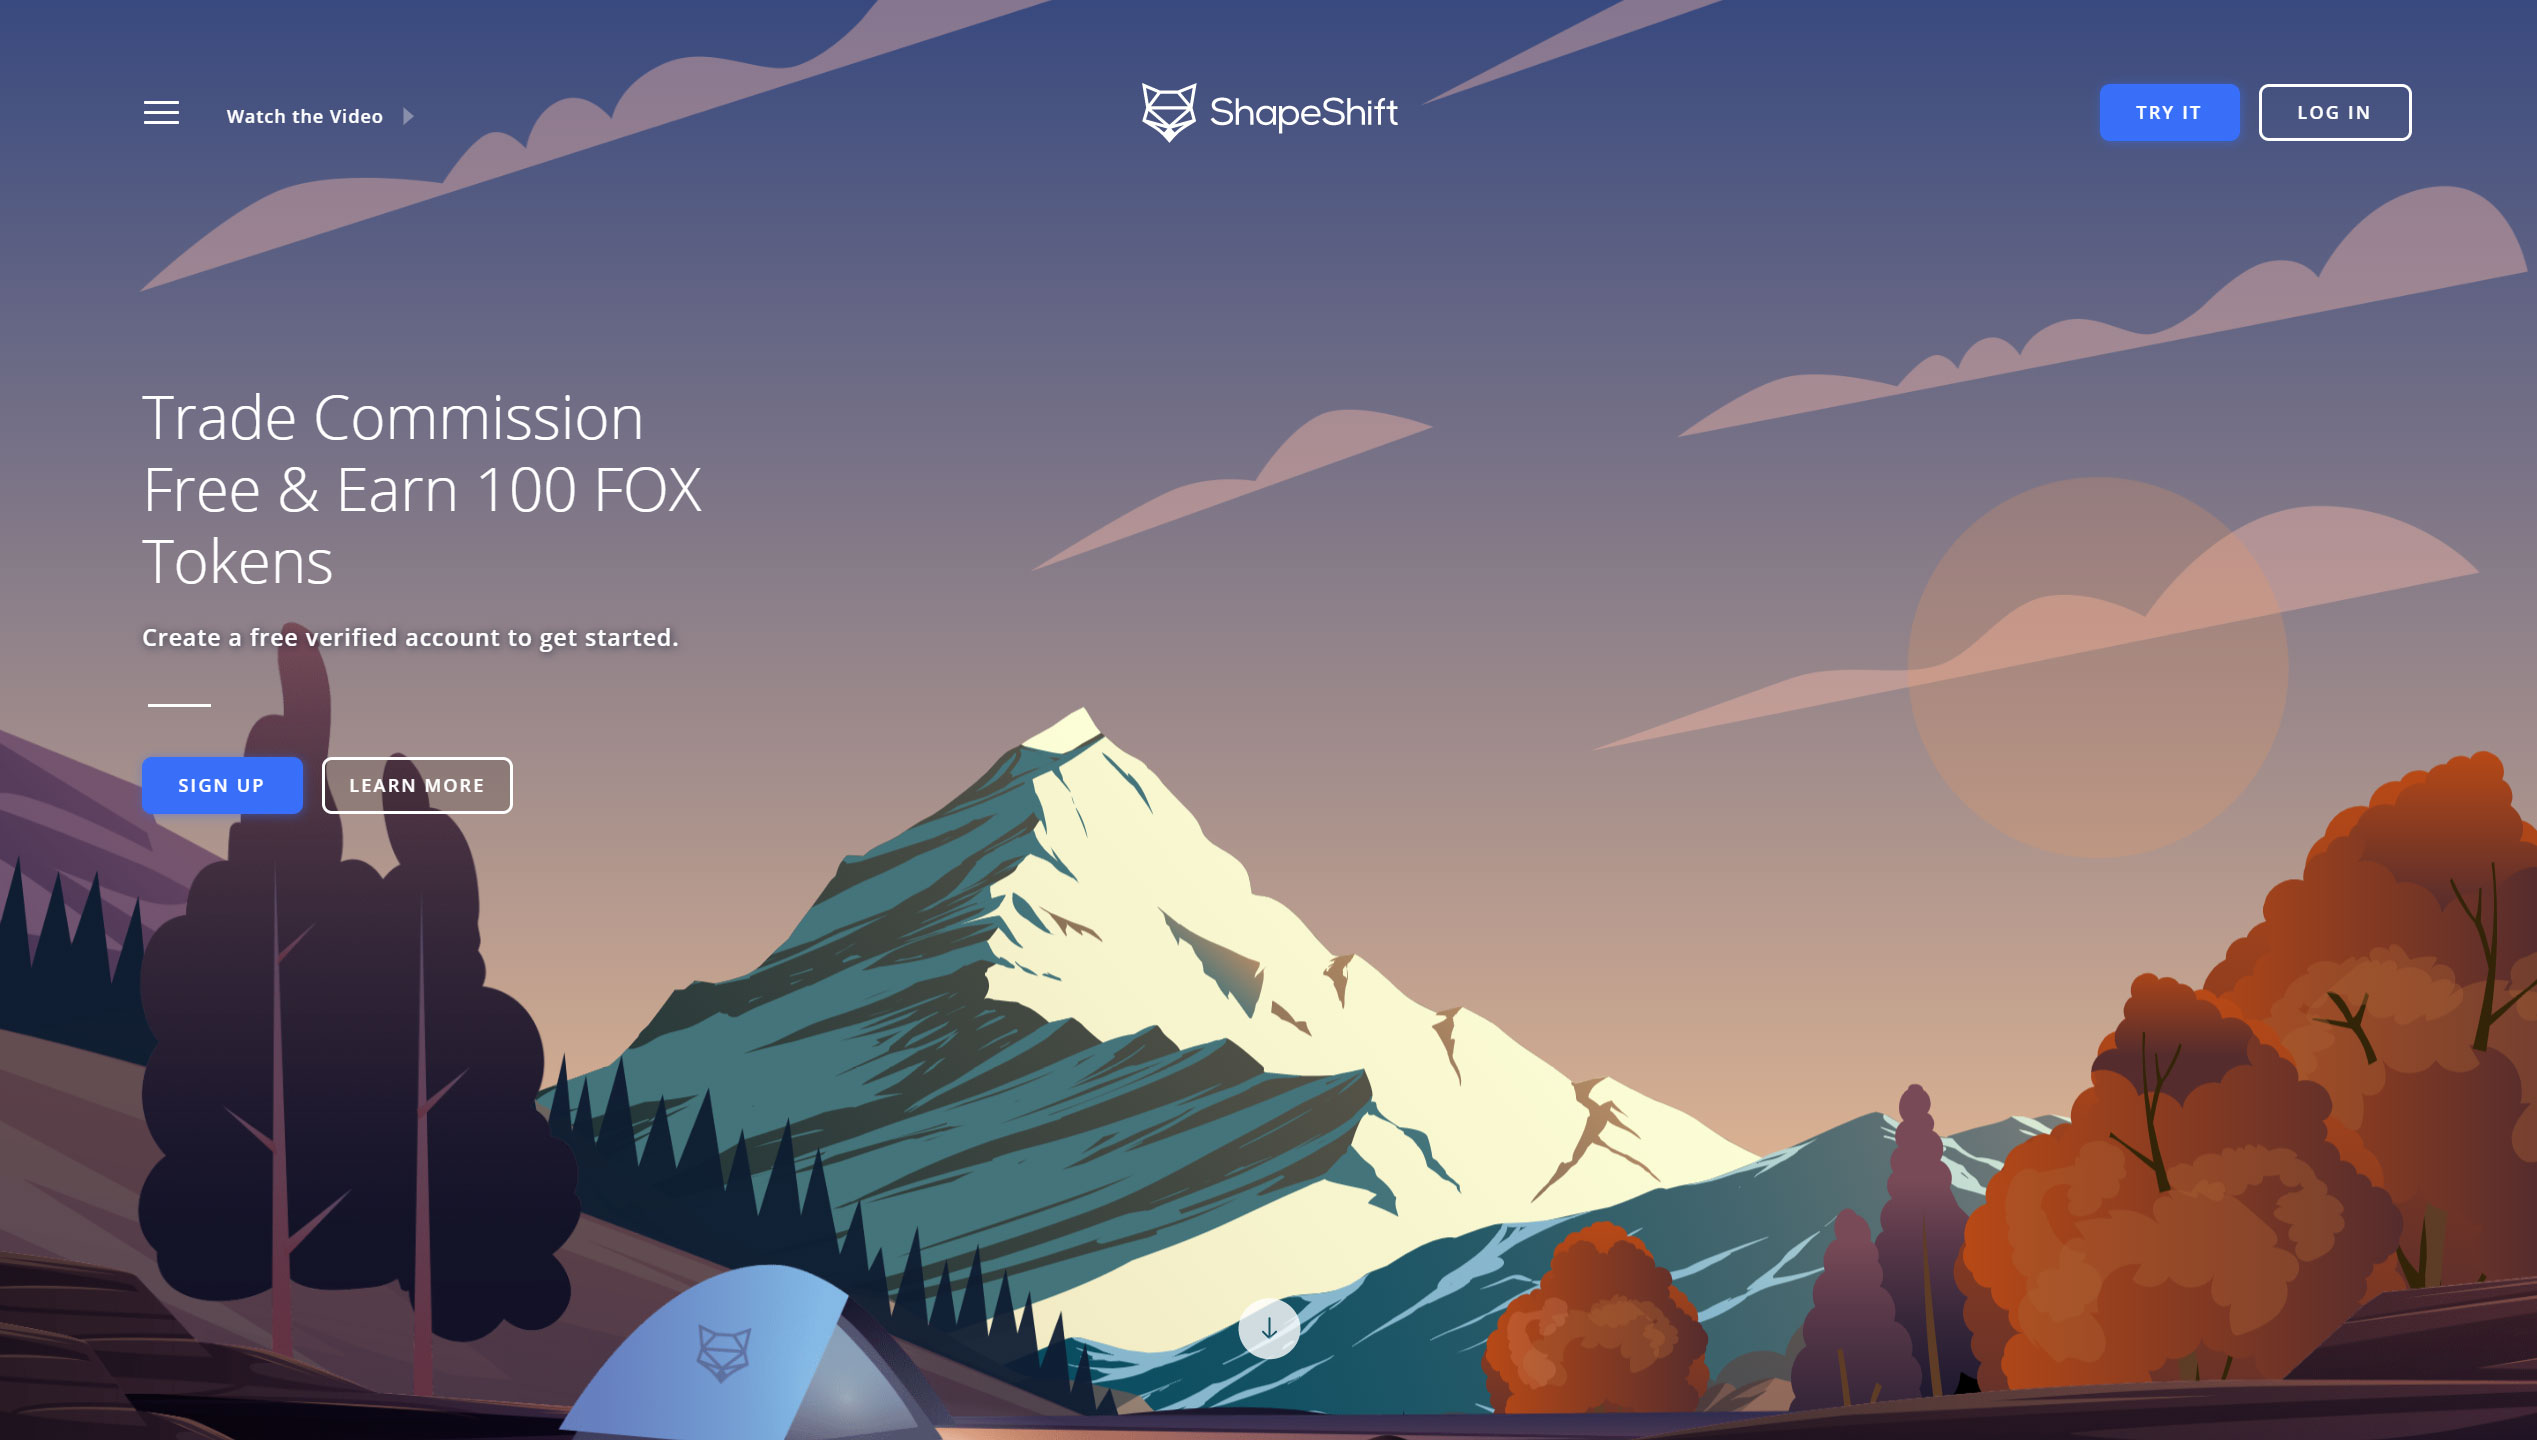
\includegraphics[width=\textwidth]{img/ch-exchanges/ShapeShift.jpg}
\end{borderbox}

\subsubsection*{Uniswap (DEX)}
Decentrale exchanges hebben het afgelopen jaar een enorme groei doorgemaakt. De interesse in DEX groeide naar aanleiding van de trend, meer beschikbaarheid en geen KYC vereisten (meer anonimiteit). Voorbeelden van gedecentraliseerde exchanges zijn Uniswap, Curve Finance, Compound, 0x Protocol, Kyber Network en nog veel meer. Momenteel is \href{https://uniswap.org}{Uniswap} verreweg het meestgebruikte gedecentraliseerde platform.


\subsubsection*{Kyber Network (DEX)}
\href{https://www.kyber.network}{Kyber Network} is een on-chain protocol waarmee iedereen instant cryptocurrencies en tokens kan inwisselen. Zo zorgt het Kyber Network ervoor dat je betalingen van bijvoorbeeld Bitcoin of Monero kan ontvangen in Ether (ETH) of andere digitale munten zonder vertraging in de transactie, en tegen kosten die bijna nihil zijn. Dit maakt de totale markt veel flexibeler en minder afhankelijk van Bitcoin (BTC) en centrale exchanges. Naarmate er meer functies komen, het handelsvolume toeneemt, en er ondersteuning voor meer cryptocurrencies komt, zal het steeds nuttiger worden voor mensen met cryptocurrency investeringen.\medskip

\begin{borderbox}
    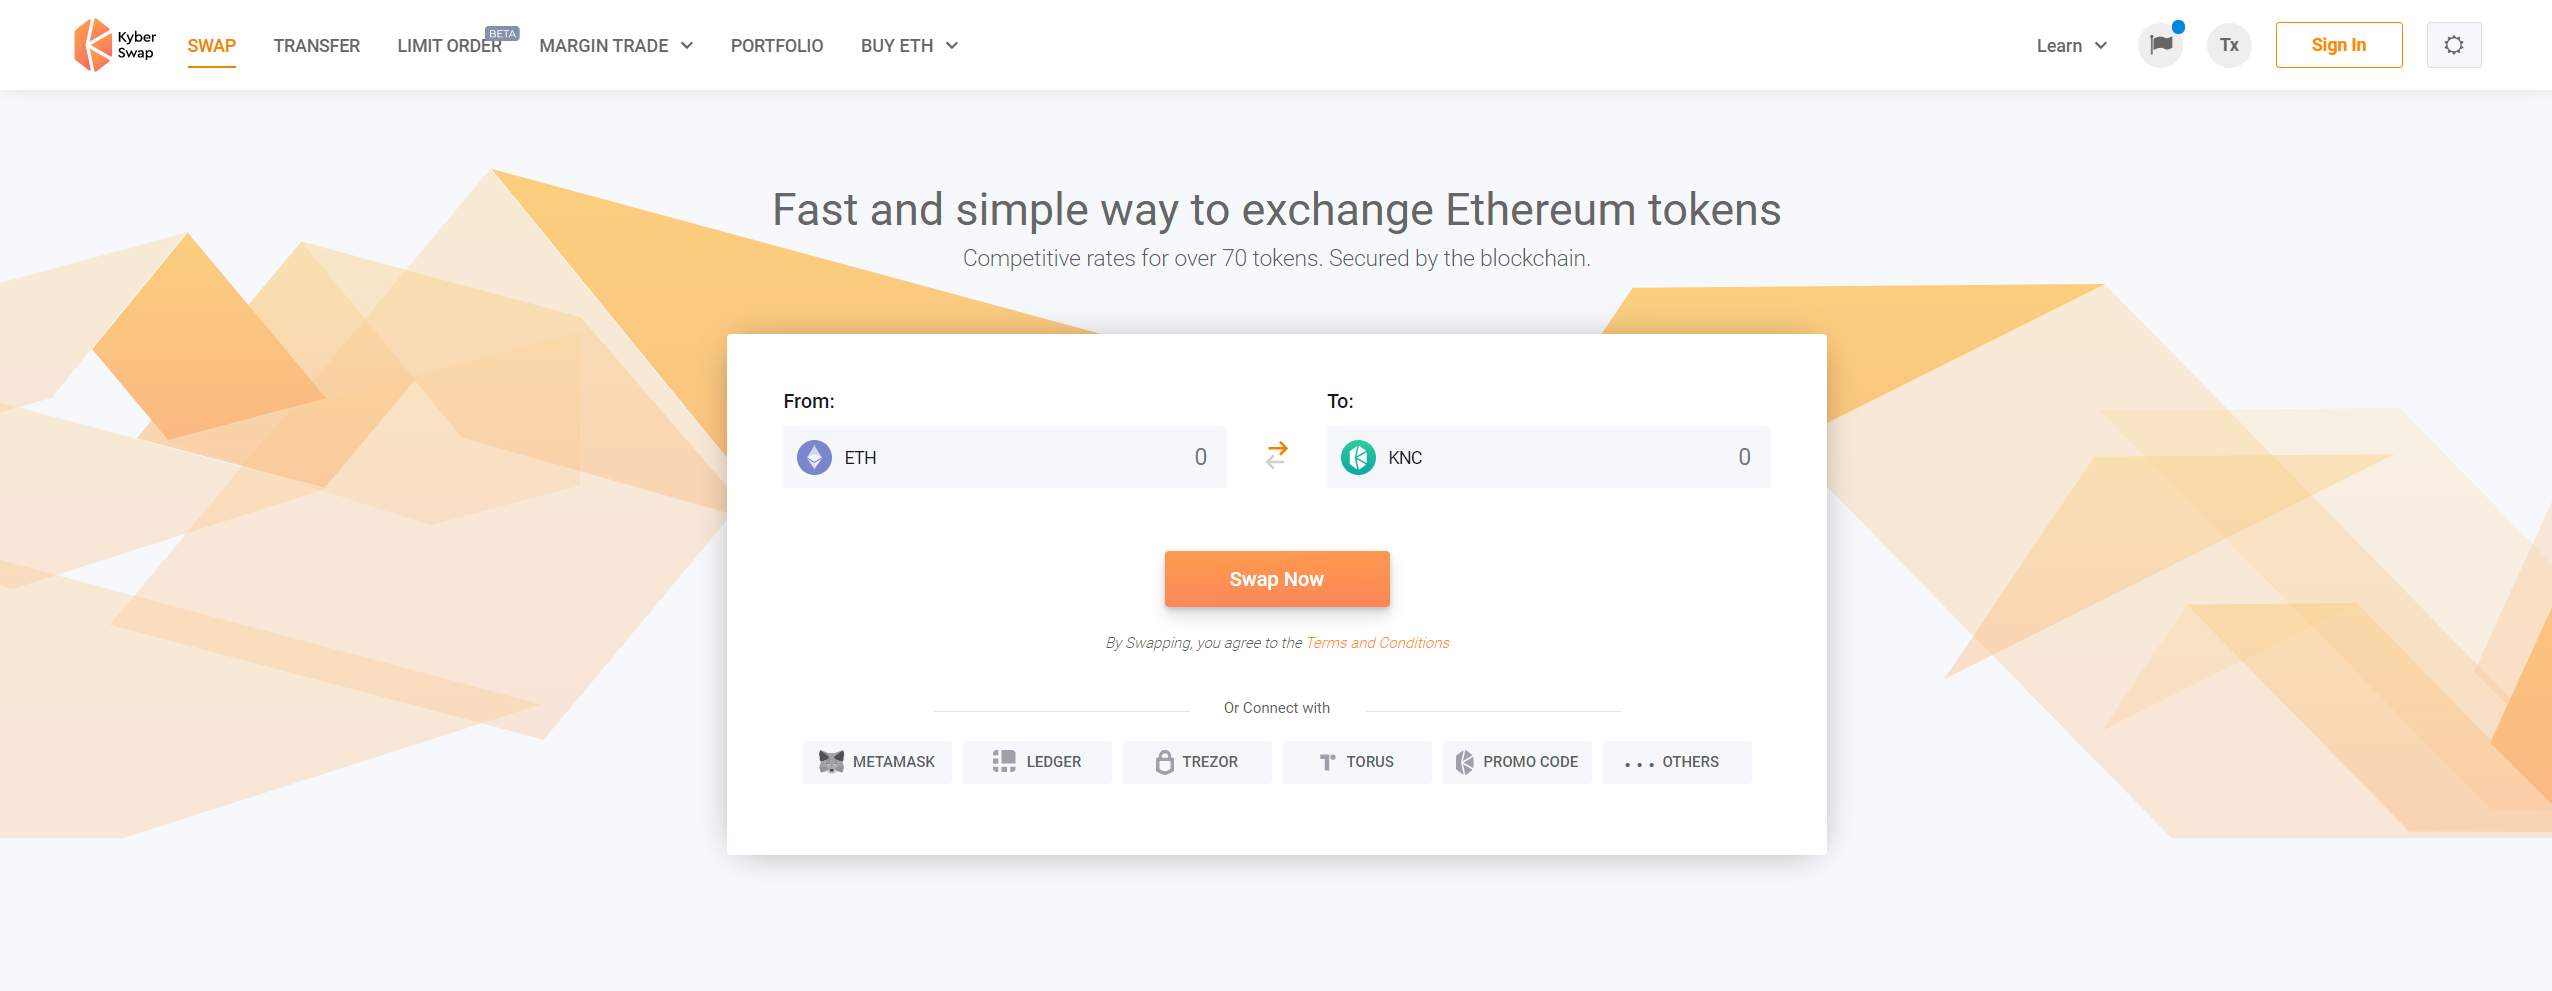
\includegraphics[width=\textwidth]{img/ch-exchanges/kyber_swap.png}
\end{borderbox}

\newpage

%\section{Broker exchanges: van fiat naar cryptocurrency}
%Eenmaal geregistreerd bij een broker exchange kan de eerste stap op de cryptocurrency markt worden gezet. Het aanbod kan per exchange verschillen en is afhankelijk van de gekozen exchange zelf, het land waar de exchange gevestigd is en de lokale regels en wetgeving die daar geldt. Het is aannemelijk dat men kiest voor een internationale broker exchange die meerdere handelsparen aanbiedt. Een andere optie kan zijn; een lokale exchange die alleen in jouw nationale currency handelt. Handelsparen die je bijna overal zult vinden zijn Bitcoin en Ethereum voor de Amerikaanse Dollar en Euro (USD/BTC, USD/ETH, EUR/BTC en EUR/ETH). Over het algemeen kan bij elke broker exchange op meerdere manieren geld worden gestort. Denk hierbij aan iDeal, PayPal, bankdeposito's (SEPA), creditcards en PayPal. Bekijk de beschikbare handelsparen en de manieren waarop geld gestort kan worden bij de gekozen broker exchange. \medskip

%\section{Trading exchanges: van crypto naar crypto}
%Indien je meerdere cryptocurrencies zou willen kopen kan het voor de nieuwkomer in het begin vrij lastig zijn om alles uit te zoeken en om de juiste infrastructuur te bepalen. Niet alle exchanges accepteren namelijk fiat currency stortingen, zoals broker exchanges dat doen. En trading exchanges staan je daarentegen vaak alleen toe om cryptocurrencies te storten om daar vervolgens andere alternatieve cryptocurrencies (altcoins) mee te verhandelen. Vervolgens is de exchange weer niet de beste plek om je cryptocurrency te bewaren.
%Vandaag de dag is Bitcoin nog steeds {\'e}{\'e}n van de meest populaire cryptocurrencies, en alle exchanges bieden dus ook Bitcoin aan. Hierdoor kun je met Bitcoin de meeste altcoins kopen. Je kunt Bitcoin, samen met Ethereum en enkele anderen, beschouwen als de beste toegangspoorten voor de aankoop van andere cryptocurrencies. 

\section{Centrale \& decentrale exchanges}
\label{sec:centralizedvsdecentralized}
In de wereld van cryptocurrencies worden exchanges voornamelijk onderverdeeld in gedecentraliseerde exchanges (DEX) en gecentraliseerde exchanges (CEX). Toonaangevende exchanges zoals Binance, Coinbase en Huobi zijn allemaal gecentraliseerd van aard. Enerzijds hebben deze een groot platform, hoog gebruikersgemak en zijn makkelijk te gebruiken. Anderzijds kunnen gecentraliseerde exchanges te kampen krijgen met veiligheidsproblemen gerelateerd aan de centrale beveiliging-structuur, waarbij de exchange de bewaarder is van jouw private keys. Gedecentraliseerde exchanges zijn - hoewel zeer veilig - nog niet heel populair bij het grote publiek. Daarvoor vergen ze meer informatie voorziening en gebruiksvriendelijkheid, wat meer gebruikers aantrekt. Wat de ontwikkeling van gedecentraliseerde exchanges betreft, moeten er nog steeds compromissen worden gesloten, zoals weergegeven in \cref{tab:centralizedvsdecentralized}. De ontwikkelingen gaan echter in hoog tempo door en er wordt gewerkt aan decentralisatie, met de gemakken van centralisatie. Dit is vooralsnog een kwestie van tijd. \medskip



\begin{table}[htb]

\centering

\caption{Centrale versus Decentrale Exchanges}
\begin{tabular}{lcl} 
\toprule
\textbf{Decentraal}         & & \textbf{Centraal}                 \\
\midrule
Gebruiker beheerd eigen fondsen       &$\longleftrightarrow$      & Exchange beheerd fondsen              \\
Anoniem            &$\longleftrightarrow$           & Niet anoniem                        \\
Weinig hacks &$\longleftrightarrow$  & Hacks mogelijk  \\
Weinig downtime &$\longleftrightarrow$  & downtime mogelijk  \\
Nog niet gebruiksvriendelijk    &$\longleftrightarrow$     & Gebruiksvriendelijk                 \\
Lager handelsvolume (illiquiditeit) &$\longleftrightarrow$ & Hoog handelsvolume (liquiditeit)              \\
Weinig handelsopties en tools &$\longleftrightarrow$ & Uitgebreide opties en tools           \\
\bottomrule
\end{tabular}
\label{tab:centralizedvsdecentralized}
\end{table}



\subsection*{Decentrale exchanges (DEX)}
\label{subsubsec:DEX}

Een decentrale exchange (DEX) is een exchange die het mogelijk maakt om cryptocurrency te traden met andere mensen die direct gebruikmaken van de blockchain. In tegenstelling tot een gecentraliseerde exchange heb je bij een DEX geen tussenpersoon nodig: er is geen centrale autoriteit of hoofd-server nodig om een transactie uit te voeren. Je kunt een DEX op dezelfde manier gebruiken als een gecentraliseerde exchange, hoewel ze meestal een lager trading volume (minder kopers en verkopers) hebben en wellicht iets minder gebruiksvriendelijk zijn qua online omgeving \& gebruikers ervaring (\say{User Interface} \& \say{User Experience}). De sector verandert echter snel naarmate de technologie verder evolueert en daardoor ontstaan er steeds betere decentrale exchanges, die gebruik maken van nieuwe (combinaties van) technologie.

\medskip

\begin{cryptobox}{BE YOUR OWN CENTRAL BANK}
    Wanneer je geen controle hebt over je private keys en in plaats daarvan je geld in een \emph{hot wallet} op een externe account - bijvoorbeeld die van Coinbase - laat opslaan, ben je in principe geen eigenaar van jouw cryptocurrencies en loop je de daaraan verbonden - en tevens onnodige - risico's. Door een deel van jouw vermogen, gerekend in traditioneel geld, om te zetten in cryptocurrencies, kun je activa zo opslaan dat alleen jij er toegang toe hebt. Zo heb je op elk moment volledige controle, zonder tegenpartijrisico (counterparty risk).
    
    \tcblower
    Remember; \textbf{not your keys - not your Crypto.}
\end{cryptobox}

\medskip

\subsection*{Centrale exchanges (CEX)}
\label{subsubsec:CEX}
Gecentraliseerde exchanges vormen de zwakste schakel in de cryptocurrency-community en een \say{chain} is slechts zo sterk als zijn zwakste \say{block}. Ironisch genoeg zijn de meeste bestaande digitale currency exchanges die binnen het cryptocurrency-ecosysteem zijn opgebouwd, gecentraliseerd. Een gecentraliseerde exchange, zoals Coinbase, Kraken of Binance, wordt gerund door een bedrijf dat zijn inkomsten haalt uit de vergoedingenstructuur [fees] die op het platform wordt gehanteerd. Zowel de entry- als de exitpunten in het huidige blockchain-ecosysteem vragen fees, die allemaal naar de gecentraliseerde exchanges gaan die deze diensten faciliteren. De afhankelijkheid en het risico dat hierdoor ontstaat en de hoge tarieven die worden aangerekend, vormen de belangrijkste redenen waarom decentrale exchanges in opkomst zijn, en ook hard nodig dus. Daarbij is het wel vermeldenswaard dat veel gecentraliseerde exchanges transacties van fiat currency naar cryptocurrency kunnen uitvoeren, terwijl gedecentraliseerde partijen meestal alleen crypto-naar-crypto transacties ondersteunen.

\medskip

Een account aanmaken voor een centrale exchange kan omslachtig zijn, vooral vanwege Know Your Customer (KYC), Anti-Money Laundering (AML), Combating the Financing of Terrorism(CFT) en andere regelgeving inzake de koppeling met traditionele financi{\"e}le infrastructuren. Wij gaan hier verder in dit hoofdstuk op in (\cref{sec:exchange-security}). 



\section{Aanmelden bij exchanges}
\label{sec:exchange-sign-up}
Het aanmelden bij een exchange is vergelijkbaar met het registreren voor een andere online betaaldienst waar je een online profiel of account moet aanmaken. Eerst zal de juiste exchange gekozen moeten worden. Neem dus de tijd om vertrouwd te geraken met de verschillende soorten exchanges, hun diensten en de voor- en nadelen. Raadpleeg \cref{sec:exchangetypes} als je niet zeker weet wat voor soort exchange je nodig hebt. In veel gevallen zul je op een bepaald punt komen dat je meerdere exchange accounts nodig hebt. 

Indien je gelijk wilt starten met het aankopen, ruilen en verkopen van cryptocurrencies, dan kun je de volgende stappen nemen:


\subsection*{Broker account openen}
\begin{enumerate}

    \item Open een exchange account en doorloop alle nodige stappen om het account te verifi{\"e}ren. Raadpleeg voor meer informatie over het "Know Your Customer" (KYC) protocol in \cref{par:KYC}.
    
    \item Stort geld van je bankrekening naar je broker exchange account. Elke exchange biedt verschillende mogelijkheden aan om geld te storten.
    
    \item Je krijgt een melding zodra het geld is aangekomen. Nu kun je Bitcoin, Ethereum of een andere cryptocurrency kopen. Let hierbij op de hoeveelheid handelsparen en handelsvolume van de exchange.\medskip
    
\begin{tipbox}{Tip}
          Indien het de bedoeling is cryptocurrency aan te kopen als investering, hoeft niet direct een account bij een trading exchange aangemaakt te worden. Veel broker exchanges bieden tegenwoordig al redelijk veel handelsparen aan. In dit geval kan de nieuw aangekochte cryptocurrency eventueel ook direct naar een (hardware) wallet gestuurd worden. Meer over hardware wallets in \cref{ch:wallets}.
\end{tipbox}
 
 \end{enumerate}
 
 \subsection*{Trading account openen}
 \begin{enumerate}[resume]
    \item Open een trading exchange account bij een exchange welke een divers aantal andere handelsparen in cryptocurrencies biedt. Meestal accepteren deze exchanges dus geen fiat currency stortingen en staan ze alleen toe om te handelen in cryptocurrencies onderling. Zie \cref{subsec:trading_exchange} voor meer informatie over trading exchanges.
    
    \item Nadat het account is geverifieerd, kan de gekochtte cryptocurrency van het broker account worden verstuurd naar het account op de nieuwe trading exchange account. Vervolgens kan met beginnen met traden. 
    
    \item  Het overgrote deel van de gekochte cryptocurrencies direct overboeken om het veilig te bewaren, raadpleeg dan \cref{ch:wallets} waar wallet en de cryptocurrency transacties verder worden besproken.
\end{enumerate}


\section{Regulering van cryptocurrency exchanges}
\label{sec:exchange-security}
Wereldwijd willen regelgevers en wetgevers er zeker van zijn dat cryptocurrency exchanges zowel de beste beveiligingspraktijken als maatregelen tegen illegale activiteiten toepassen. Deze maatregelen ontmoedigen illegale activiteiten en verbeteren daarnaast de online veiligheid van centrale exchange accounts en de daarbij behorende cryptocurrency wallets. 

\begin{enumerate}
    \item \emph{Know Your Customer} (KYC)
    \item \emph{Anti Money Laundering} (AML)
    \item \emph{Combating the Financing of Terrorism} (CFT)
\end{enumerate} 

Het is belangrijk om te weten waar ze voor staan, omdat je er hoe dan ook mee te maken krijgt zodra jij een account aanmaakt bij een exchange. Dan weet je ook waarom al deze informatie opgevraagd wordt en waarom al deze stappen worden doorlopen bij het openen van een centrale exchange account.


\subsection*{Know Your Customer (KYC)}
\label{par:KYC}
KYC verwijst naar een set voorschriften, procedures en processen die exchanges gebruiken om de identiteit van hun klanten te achterhalen. Wanneer je fiat currency stort om aankopen te doen en vervolgens te traden, moet je vrijwel altijd je identiteit verifi{\"e}ren. Deze verificatie kan op verschillende manieren, afhankelijk van de nationaliteit en gekozen exchange. Het houdt vaak in dat je een foto van jezelf met je ID, paspoort, rijbewijs, of andere offici{\"e}le documentatie moet uploaden voor je toegang krijgt.\medskip

Voor lage geldbedragen is dit mogelijk geen vereiste - en is er een verschil tussen broker en trading- exchanges (\cref{subsubsec:DEX} \& \cref{subsubsec:CEX}) - maar ben je van plan om regelmatig grotere hoeveelheden geld te storten en op te nemen, dan kan het nodig zijn om verschillende verificatiefasen te doorlopen. Toegang tot een hoger niveau vertaalt zich in het uploaden van bijkomende persoonlijke documenten zoals bankafschriften of een huurovereenkomst. Dit gehele proces wordt meestal aangeduid als KYC (Know Your Customer).

\subsection*{Anti-Money Laundering (AML)}
AML omslaat een reeks procedures, wetten en voorschriften die als doel hebben om een einde te maken aan illegale activiteiten zoals het witwassen van geld. Sommigen van hen omvatten belastingontduiking, marktmanipulatie, verduistering van openbare middelen, handel in illegale goederen en andere activiteiten van deze aard.

AML-voorschriften verplichten financi{\"e}le instellingen om voortdurend \emph{due diligence}-procedures uit te voeren om kwaadaardige activiteiten op te sporen en te voorkomen.

\subsection*{Combating the Financing of Terrorism (CFT)}
CFT verwijst naar de reeks procedures die gericht zijn op het onderzoeken, ontleden, ontmoedigen en blokkeren van financieringsbronnen voor activiteiten die mogelijk gelinkt zijn met terrorisme. Deze financiering is dan bedoeld voor activiteiten die religieuze, ideologische of politieke doelen verwezenlijken door geweld, of de dreiging daarvan, tegen burgers. Deze set van CFT procedures bieden instanties een alternatieve en mogelijk effectieve manier om terroristische activiteiten in de financi{\"e}le sector op te sporen en te blokkeren.



\section{\emph{Best Practices} - crypto exchanges}
\label{sec:importantconsiderations}
De {\fontseries{extrabold}\selectfont Cryptomanual} \say{{\fontseries{medium}\selectfont Best Practices}} verschaft natuurlijk een aantal aandachtspunten en een set aanbevelingen waar men op kan letten bij het kiezen van exchange(s). Allereerst zijn in \cref{tab:exchangeoverview} een aantal exchanges opgenomen waarmee voor iedereen de basis prima gedekt zou moeten zijn. Indien er alsnog de behoefte is om de minder toegankelijke crypto te kopen, moeten er meerdere exchange-accounts worden aangemaakt, simpelweg omdat het aanbod van exchanges onderling zo verschilt. De volgende punten kun je op letten:

\begin{table}[b]

\centering

\caption{Aanbevolen \emph{broker} en \emph{trading} exchanges}
\begin{tabular}{llll} 
\toprule

\textbf{Exchange} & \textbf{Type } & \textbf{UX/UI} & \textbf{URL}\\
\midrule

Coinbase & Broker & Beginner & \href{https://www.coinbase.com/join/51954a2b26a1bcc484000015}{coinbase.com} \\
KuCoin   &  Trading & Beginner & \href{https://www.kucoin.com/#/?r=aNuPeb}{intro.kucoin.com} \\
Binance  &  Trading & Beginner & \href{https://www.binance.com/?ref=35602166}{binance.com} \\
Liquid   &  Broker/Trading & Beginner & \href{https://www.liquid.com?affiliate=nUfQhVL4164547}{liquid.com} \\
Kraken   &  Broker/Trading & Intermediate & \href{https://www.kraken.com/}{kraken.com} \\


\bottomrule
\end{tabular}
\label{tab:exchange selection}
\end{table}

\subsection*{Handelsvolume \& liquiditeit}
Hou rekening met de grootte van de exchange. Hoe groter de exchange, hoe meer cryptocurrencies er worden verhandeld, en hoe hoger het handelsvolume. Over het algemeen geldt, hoe hoger het dagelijks handelsvolume, hoe makkelijker jij kan aan- en verkopen.

\subsection*{Handelsparen}
Tegelijk kijk je ook naar wat invloed heeft op dat handelsvolume, zoals de beschikbare opties in \emph{trading pairs} oftewel handelsparen zoals: USD/BTC, USD/ETH, EUR/BTC en EUR/ETH. Bitcoin (BTC) domineert de cryptocurrencymarkt tot op heden, maar er zijn genoeg andere cryptocurrencies - zoals Ethereum - met enorme handelsvolumes over periodes van 24 uur.

\medskip 
\begin{borderbox}
    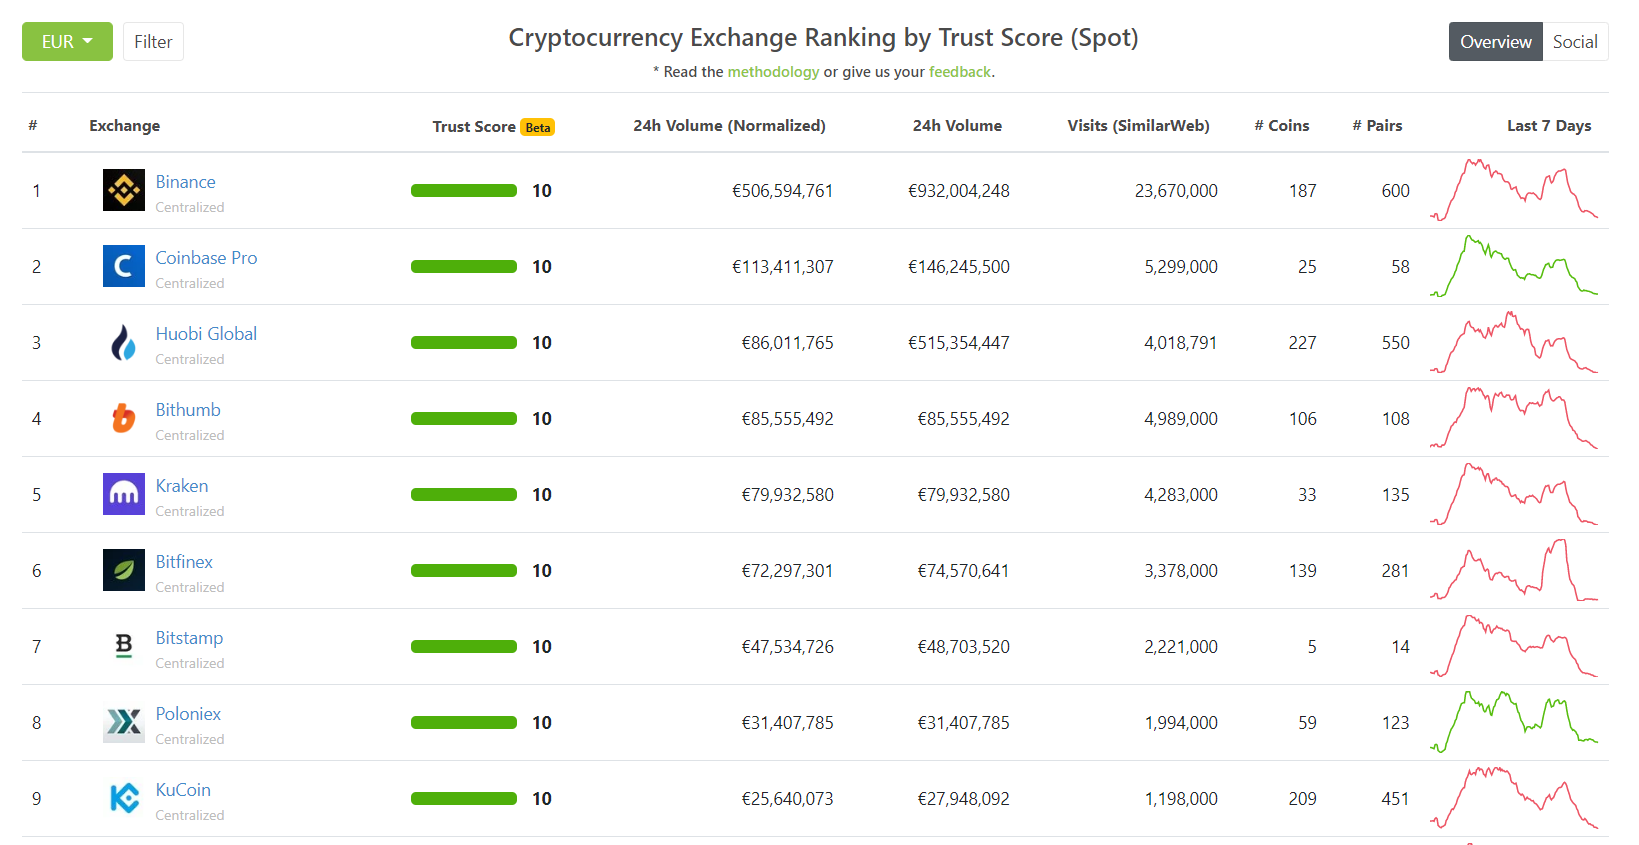
\includegraphics[width=\textwidth]{img/ch-exchanges/exchange-ranking.png}
\end{borderbox}
\medskip

\subsection*{Reputatie} Zoek naar reviews van individuele gebruikers en betrouwbare partijen in de industrie. Daarnaast kun je vragen stellen op offici{\"e}le sociale media of aan de community op bijvoorbeeld Telegram.

\subsection*{Geografische Beperkingen}  Het kan zijn dat er lokaal andere wettelijke verplichtingen of regels gelden. Sommige specifieke gebruikers-functies die door exchanges worden aangeboden, zijn alleen toegankelijk vanuit bepaalde landen. Zorg ervoor dat de exchange waar jij je zou willen aanmelden, volledige toegang biedt tot alle functies en diensten waar je gebruik van wilt maken, zo kom je later niet voor rare verassingen te staan. 

\subsection*{Betaalwijze} Kijk goed naar welke betaalwijzen beschikbaar zijn. Denk hierbij aan incasso's, krediet- en debetkaarten, bank overschrijvingen, PayPal en natuurlijk cryptocurrencies. Wanneer een broker exchange beperkte betalingsmogelijkheden aanbiedt, dan is het voor jou wellicht niet handig om deze broker exchange te gebruiken. Vergeet niet dat voor de aankoop van cryptocurrencies met een creditcard altijd een identiteit-verificatie nodig is en dat er vaak hogere transactie- en verwerkingskosten betaald worden. Het kopen van cryptocurrency via een bankoverschrijving zal aanzienlijk langer duren omdat het voor banken met een klassieke infrastructuur wellicht enkele dagen duurt om deze transactie te verwerken.

\subsection*{Verificatie-eisen} De overgrote meerderheid van de exchanges in zowel de VS als het Verenigd Koninkrijk eisen enige ID-verificatie nodig om stortingen en opnames te kunnen doen. Sommige exchanges staan het toe om anoniem te blijven. Hoewel de verificatie, die tot een paar dagen kan duren, misschien een pijnlijke zaak lijkt, beschermt het de exchange enigzins tegen vormen van oplichterij en het witwassen van geld. Het nadeel is dat de poort naar cryptocurrencies vaak niet anoniem kan plaatsvinden, terwijl dat een van de aantrekkelijke eigenschappen is van de vele \emph{privacy coins}.


\subsection*{Fees} Afhankelijk van de exchange die je gebruikt, kunnen de kosten aanzienlijk verschillen. Informeer je goed over de storting-, transactie- en opnamekosten voordat je je registreert. Cryptocurrency exchanges dienen op hun website te vermelden hoeveel kosten ze in rekening brengen.  

\subsection*{Wisselkoersen} Verschillende exchanges hanteren verschillende tarieven omtrent wisselkoersen. Je zult verbaasd staan hoeveel je kunt besparen door de juiste exchange te kiezen. Het is niet ongewoon dat wisselkoersen met tien procent schommelen. Dit wordt natuurlijk steeds belangrijker als je van plan bent vaker te traden.






